\documentclass[1p]{elsarticle_modified}
%\bibliographystyle{elsarticle-num}

%\usepackage[colorlinks]{hyperref}
%\usepackage{abbrmath_seonhwa} %\Abb, \Ascr, \Acal ,\Abf, \Afrak
\usepackage{amsfonts}
\usepackage{amssymb}
\usepackage{amsmath}
\usepackage{amsthm}
\usepackage{scalefnt}
\usepackage{amsbsy}
\usepackage{kotex}
\usepackage{caption}
\usepackage{subfig}
\usepackage{color}
\usepackage{graphicx}
\usepackage{xcolor} %% white, black, red, green, blue, cyan, magenta, yellow
\usepackage{float}
\usepackage{setspace}
\usepackage{hyperref}

\usepackage{tikz}
\usetikzlibrary{arrows}

\usepackage{multirow}
\usepackage{array} % fixed length table
\usepackage{hhline}

%%%%%%%%%%%%%%%%%%%%%
\makeatletter
\renewcommand*\env@matrix[1][\arraystretch]{%
	\edef\arraystretch{#1}%
	\hskip -\arraycolsep
	\let\@ifnextchar\new@ifnextchar
	\array{*\c@MaxMatrixCols c}}
\makeatother %https://tex.stackexchange.com/questions/14071/how-can-i-increase-the-line-spacing-in-a-matrix
%%%%%%%%%%%%%%%

\usepackage[normalem]{ulem}

\newcommand{\msout}[1]{\ifmmode\text{\sout{\ensuremath{#1}}}\else\sout{#1}\fi}
%SOURCE: \msout is \stkout macro in https://tex.stackexchange.com/questions/20609/strikeout-in-math-mode

\newcommand{\cancel}[1]{
	\ifmmode
	{\color{red}\msout{#1}}
	\else
	{\color{red}\sout{#1}}
	\fi
}

\newcommand{\add}[1]{
	{\color{blue}\uwave{#1}}
}

\newcommand{\replace}[2]{
	\ifmmode
	{\color{red}\msout{#1}}{\color{blue}\uwave{#2}}
	\else
	{\color{red}\sout{#1}}{\color{blue}\uwave{#2}}
	\fi
}

\newcommand{\Sol}{\mathcal{S}} %segment
\newcommand{\D}{D} %diagram
\newcommand{\A}{\mathcal{A}} %arc


%%%%%%%%%%%%%%%%%%%%%%%%%%%%%5 test

\def\sl{\operatorname{\textup{SL}}(2,\Cbb)}
\def\psl{\operatorname{\textup{PSL}}(2,\Cbb)}
\def\quan{\mkern 1mu \triangleright \mkern 1mu}

\theoremstyle{definition}
\newtheorem{thm}{Theorem}[section]
\newtheorem{prop}[thm]{Proposition}
\newtheorem{lem}[thm]{Lemma}
\newtheorem{ques}[thm]{Question}
\newtheorem{cor}[thm]{Corollary}
\newtheorem{defn}[thm]{Definition}
\newtheorem{exam}[thm]{Example}
\newtheorem{rmk}[thm]{Remark}
\newtheorem{alg}[thm]{Algorithm}

\newcommand{\I}{\sqrt{-1}}
\begin{document}

%\begin{frontmatter}
%
%\title{Boundary parabolic representations of knots up to 8 crossings}
%
%%% Group authors per affiliation:
%\author{Yunhi Cho} 
%\address{Department of Mathematics, University of Seoul, Seoul, Korea}
%\ead{yhcho@uos.ac.kr}
%
%
%\author{Seonhwa Kim} %\fnref{s_kim}}
%\address{Center for Geometry and Physics, Institute for Basic Science, Pohang, 37673, Korea}
%\ead{ryeona17@ibs.re.kr}
%
%\author{Hyuk Kim}
%\address{Department of Mathematical Sciences, Seoul National University, Seoul 08826, Korea}
%\ead{hyukkim@snu.ac.kr}
%
%\author{Seokbeom Yoon}
%\address{Department of Mathematical Sciences, Seoul National University, Seoul, 08826,  Korea}
%\ead{sbyoon15@snu.ac.kr}
%
%\begin{abstract}
%We find all boundary parabolic representation of knots up to 8 crossings.
%
%\end{abstract}
%\begin{keyword}
%    \MSC[2010] 57M25 
%\end{keyword}
%
%\end{frontmatter}

%\linenumbers
%\tableofcontents
%
\newcommand\colored[1]{\textcolor{white}{\rule[-0.35ex]{0.8em}{1.4ex}}\kern-0.8em\color{red} #1}%
%\newcommand\colored[1]{\textcolor{white}{ #1}\kern-2.17ex	\textcolor{white}{ #1}\kern-1.81ex	\textcolor{white}{ #1}\kern-2.15ex\color{red}#1	}

{\Large $\underline{11n_{8}~(K11n_{8})}$}

\setlength{\tabcolsep}{10pt}
\renewcommand{\arraystretch}{1.6}
\vspace{1cm}\begin{tabular}{m{100pt}>{\centering\arraybackslash}m{274pt}}
\multirow{5}{120pt}{
	\centering
	\includegraphics[width=112pt]{../../../GIT/diagram.site/Diagrams/png/624_11n_8.png}\\
\ \ \ A knot diagram\footnotemark}&
\allowdisplaybreaks
\textbf{Linearized knot diagam} \\
\cline{2-2}
 &
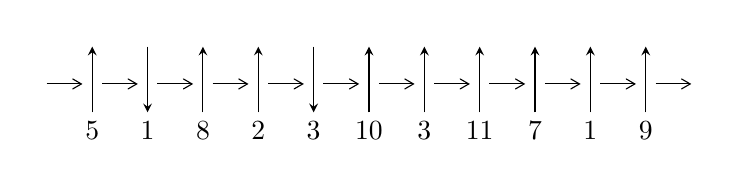
\begin{tikzpicture}[x=20pt, y=17pt]
	% nodes
	\node (C0) at (0, 0) {};
	\node (C1) at (1, 0) {};
	\node (C1U) at (1, +1) {};
	\node (C1D) at (1, -1) {5};

	\node (C2) at (2, 0) {};
	\node (C2U) at (2, +1) {};
	\node (C2D) at (2, -1) {1};

	\node (C3) at (3, 0) {};
	\node (C3U) at (3, +1) {};
	\node (C3D) at (3, -1) {8};

	\node (C4) at (4, 0) {};
	\node (C4U) at (4, +1) {};
	\node (C4D) at (4, -1) {2};

	\node (C5) at (5, 0) {};
	\node (C5U) at (5, +1) {};
	\node (C5D) at (5, -1) {3};

	\node (C6) at (6, 0) {};
	\node (C6U) at (6, +1) {};
	\node (C6D) at (6, -1) {10};

	\node (C7) at (7, 0) {};
	\node (C7U) at (7, +1) {};
	\node (C7D) at (7, -1) {3};

	\node (C8) at (8, 0) {};
	\node (C8U) at (8, +1) {};
	\node (C8D) at (8, -1) {11};

	\node (C9) at (9, 0) {};
	\node (C9U) at (9, +1) {};
	\node (C9D) at (9, -1) {7};

	\node (C10) at (10, 0) {};
	\node (C10U) at (10, +1) {};
	\node (C10D) at (10, -1) {1};

	\node (C11) at (11, 0) {};
	\node (C11U) at (11, +1) {};
	\node (C11D) at (11, -1) {9};
	\node (C12) at (12, 0) {};

	% arrows
	\draw[->,>={angle 60}]
	(C0) edge (C1) (C1) edge (C2) (C2) edge (C3) (C3) edge (C4) (C4) edge (C5) (C5) edge (C6) (C6) edge (C7) (C7) edge (C8) (C8) edge (C9) (C9) edge (C10) (C10) edge (C11) (C11) edge (C12) ;	\draw[->,>=stealth]
	(C1D) edge (C1U) (C2U) edge (C2D) (C3D) edge (C3U) (C4D) edge (C4U) (C5U) edge (C5D) (C6D) edge (C6U) (C7D) edge (C7U) (C8D) edge (C8U) (C9D) edge (C9U) (C10D) edge (C10U) (C11D) edge (C11U) ;
	\end{tikzpicture} \\
\hhline{~~} \\& 
\textbf{Solving Sequence} \\ \cline{2-2} 
 &
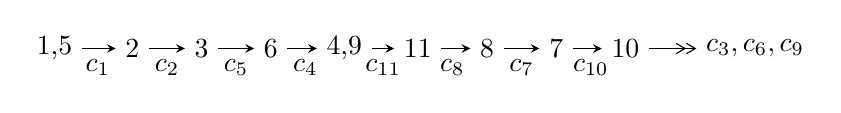
\begin{tikzpicture}[x=25pt, y=7pt]
	% node
	\node (A0) at (-1/8, 0) {1,5};
	\node (A1) at (1, 0) {2};
	\node (A2) at (2, 0) {3};
	\node (A3) at (3, 0) {6};
	\node (A4) at (65/16, 0) {4,9};
	\node (A5) at (41/8, 0) {11};
	\node (A6) at (49/8, 0) {8};
	\node (A7) at (57/8, 0) {7};
	\node (A8) at (65/8, 0) {10};
	\node (C1) at (1/2, -1) {$c_{1}$};
	\node (C2) at (3/2, -1) {$c_{2}$};
	\node (C3) at (5/2, -1) {$c_{5}$};
	\node (C4) at (7/2, -1) {$c_{4}$};
	\node (C5) at (37/8, -1) {$c_{11}$};
	\node (C6) at (45/8, -1) {$c_{8}$};
	\node (C7) at (53/8, -1) {$c_{7}$};
	\node (C8) at (61/8, -1) {$c_{10}$};
	\node (A9) at (10, 0) {$c_{3},c_{6},c_{9}$};

	% edge
	\draw[->,>=stealth]	
	(A0) edge (A1) (A1) edge (A2) (A2) edge (A3) (A3) edge (A4) (A4) edge (A5) (A5) edge (A6) (A6) edge (A7) (A7) edge (A8) ;
	\draw[->>,>={angle 60}]	
	(A8) edge (A9);
\end{tikzpicture} \\ 

\end{tabular} \\

\footnotetext{
The image of knot diagram is generated by the software ``\textbf{Draw programme}" developed by Andrew Bartholomew(\url{http://www.layer8.co.uk/maths/draw/index.htm\#Running-draw}), where we modified some parts for our purpose(\url{https://github.com/CATsTAILs/LinksPainter}).
}\phantom \\ \newline 
\centering \textbf{Ideals for irreducible components\footnotemark of $X_{\text{par}}$} 
 
\begin{align*}
I^u_{1}&=\langle 
17327884311 u^{31}-51370177786 u^{30}+\cdots+50776700428 b+45898407811,\\
\phantom{I^u_{1}}&\phantom{= \langle  }65060365722 u^{31}-300114124597 u^{30}+\cdots+50776700428 a+117492282989,\\
\phantom{I^u_{1}}&\phantom{= \langle  }u^{32}-4 u^{31}+\cdots+4 u+1\rangle \\
I^u_{2}&=\langle 
- a u+b- a+u+1,\;a^3- a^2 u-3 a^2+2 a u+3 a- u,\;u^2+u+1\rangle \\
\\
\end{align*}
\raggedright * 2 irreducible components of $\dim_{\mathbb{C}}=0$, with total 38 representations.\\
\footnotetext{All coefficients of polynomials are rational numbers. But the coefficients are sometimes approximated in decimal forms when there is not enough margin.}
\newpage
\renewcommand{\arraystretch}{1}
\centering \section*{I. $I^u_{1}= \langle 1.73\times10^{10} u^{31}-5.14\times10^{10} u^{30}+\cdots+5.08\times10^{10} b+4.59\times10^{10},\;6.51\times10^{10} u^{31}-3.00\times10^{11} u^{30}+\cdots+5.08\times10^{10} a+1.17\times10^{11},\;u^{32}-4 u^{31}+\cdots+4 u+1 \rangle$}
\flushleft \textbf{(i) Arc colorings}\\
\begin{tabular}{m{7pt} m{180pt} m{7pt} m{180pt} }
\flushright $a_{1}=$&$\begin{pmatrix}1\\0\end{pmatrix}$ \\
\flushright $a_{5}=$&$\begin{pmatrix}0\\u\end{pmatrix}$ \\
\flushright $a_{2}=$&$\begin{pmatrix}1\\- u^2\end{pmatrix}$ \\
\flushright $a_{3}=$&$\begin{pmatrix}u^2+1\\- u^2\end{pmatrix}$ \\
\flushright $a_{6}=$&$\begin{pmatrix}- u^5-2 u^3- u\\u^5+u^3+u\end{pmatrix}$ \\
\flushright $a_{4}=$&$\begin{pmatrix}- u\\u^3+u\end{pmatrix}$ \\
\flushright $a_{9}=$&$\begin{pmatrix}-1.28130 u^{31}+5.91047 u^{30}+\cdots-2.94899 u-2.31390\\-0.341257 u^{31}+1.01169 u^{30}+\cdots-2.34798 u-0.903927\end{pmatrix}$ \\
\flushright $a_{11}=$&$\begin{pmatrix}0.466042 u^{31}-2.36981 u^{30}+\cdots+6.05202 u+2.89832\\-0.115026 u^{31}+0.296752 u^{30}+\cdots+0.358069 u+0.384294\end{pmatrix}$ \\
\flushright $a_{8}=$&$\begin{pmatrix}-0.710734 u^{31}+3.43037 u^{30}+\cdots-0.0540527 u-1.07276\\-0.587434 u^{31}+1.13312 u^{30}+\cdots-1.77017 u-0.710734\end{pmatrix}$ \\
\flushright $a_{7}=$&$\begin{pmatrix}-1.23870 u^{31}+3.83973 u^{30}+\cdots-2.78410 u-1.05967\\0.352028 u^{31}-0.853772 u^{30}+\cdots-1.08485 u-0.642279\end{pmatrix}$ \\
\flushright $a_{10}=$&$\begin{pmatrix}0.581069 u^{31}-2.66656 u^{30}+\cdots+5.69396 u+2.51403\\-0.115026 u^{31}+0.296752 u^{30}+\cdots+0.358069 u+0.384294\end{pmatrix}$\\ \flushright $a_{10}=$&$\begin{pmatrix}0.581069 u^{31}-2.66656 u^{30}+\cdots+5.69396 u+2.51403\\-0.115026 u^{31}+0.296752 u^{30}+\cdots+0.358069 u+0.384294\end{pmatrix}$\\&\end{tabular}
\flushleft \textbf{(ii) Obstruction class $= -1$}\\~\\
\flushleft \textbf{(iii) Cusp Shapes $= \frac{19161957911}{12694175107} u^{31}-\frac{109525992335}{25388350214} u^{30}+\cdots+\frac{73849369350}{12694175107} u+\frac{129286515817}{12694175107}$}\\~\\
\newpage\renewcommand{\arraystretch}{1}
\flushleft \textbf{(iv) u-Polynomials at the component}\newline \\
\begin{tabular}{m{50pt}|m{274pt}}
Crossings & \hspace{64pt}u-Polynomials at each crossing \\
\hline $$\begin{aligned}c_{1},c_{4}\end{aligned}$$&$\begin{aligned}
&u^{32}+4 u^{31}+\cdots-4 u+1
\end{aligned}$\\
\hline $$\begin{aligned}c_{2}\end{aligned}$$&$\begin{aligned}
&u^{32}+8 u^{31}+\cdots-4 u+1
\end{aligned}$\\
\hline $$\begin{aligned}c_{3},c_{7}\end{aligned}$$&$\begin{aligned}
&u^{32}+3 u^{31}+\cdots-32 u+64
\end{aligned}$\\
\hline $$\begin{aligned}c_{5}\end{aligned}$$&$\begin{aligned}
&u^{32}-4 u^{31}+\cdots-5956 u+3137
\end{aligned}$\\
\hline $$\begin{aligned}c_{6},c_{9}\end{aligned}$$&$\begin{aligned}
&u^{32}+3 u^{31}+\cdots-3 u-1
\end{aligned}$\\
\hline $$\begin{aligned}c_{8},c_{11}\end{aligned}$$&$\begin{aligned}
&u^{32}+3 u^{31}+\cdots+5 u-1
\end{aligned}$\\
\hline $$\begin{aligned}c_{10}\end{aligned}$$&$\begin{aligned}
&u^{32}-21 u^{31}+\cdots-11 u+1
\end{aligned}$\\
\hline
\end{tabular}\\~\\
\newpage\renewcommand{\arraystretch}{1}
\flushleft \textbf{(v) Riley Polynomials at the component}\newline \\
\begin{tabular}{m{50pt}|m{274pt}}
Crossings & \hspace{64pt}Riley Polynomials at each crossing \\
\hline $$\begin{aligned}c_{1},c_{4}\end{aligned}$$&$\begin{aligned}
&y^{32}+8 y^{31}+\cdots-4 y+1
\end{aligned}$\\
\hline $$\begin{aligned}c_{2}\end{aligned}$$&$\begin{aligned}
&y^{32}+36 y^{31}+\cdots-400 y+1
\end{aligned}$\\
\hline $$\begin{aligned}c_{3},c_{7}\end{aligned}$$&$\begin{aligned}
&y^{32}-35 y^{31}+\cdots-50176 y+4096
\end{aligned}$\\
\hline $$\begin{aligned}c_{5}\end{aligned}$$&$\begin{aligned}
&y^{32}+64 y^{31}+\cdots+37894220 y+9840769
\end{aligned}$\\
\hline $$\begin{aligned}c_{6},c_{9}\end{aligned}$$&$\begin{aligned}
&y^{32}+3 y^{31}+\cdots-11 y+1
\end{aligned}$\\
\hline $$\begin{aligned}c_{8},c_{11}\end{aligned}$$&$\begin{aligned}
&y^{32}-21 y^{31}+\cdots-11 y+1
\end{aligned}$\\
\hline $$\begin{aligned}c_{10}\end{aligned}$$&$\begin{aligned}
&y^{32}-17 y^{31}+\cdots+225 y+1
\end{aligned}$\\
\hline
\end{tabular}\\~\\
\newpage\flushleft \textbf{(vi) Complex Volumes and Cusp Shapes}
$$\begin{array}{c|c|c}  
\text{Solutions to }I^u_{1}& \I (\text{vol} + \sqrt{-1}CS) & \text{Cusp shape}\\
 \hline 
\begin{aligned}
u &= -0.438343 + 0.910233 I \\
a &= -1.25471 + 2.63396 I \\
b &= -0.961368 + 0.135359 I\end{aligned}
 & \phantom{-}1.31776 - 2.35125 I & \phantom{-}21.8207 - 1.6456 I \\ \hline\begin{aligned}
u &= -0.438343 - 0.910233 I \\
a &= -1.25471 - 2.63396 I \\
b &= -0.961368 - 0.135359 I\end{aligned}
 & \phantom{-}1.31776 + 2.35125 I & \phantom{-}21.8207 + 1.6456 I \\ \hline\begin{aligned}
u &= -0.607222 + 0.839985 I \\
a &= -0.488594 + 0.148224 I \\
b &= -0.225556 + 0.193839 I\end{aligned}
 & \phantom{-}0.60688 - 2.35983 I & \phantom{-}1.68069 + 4.72936 I \\ \hline\begin{aligned}
u &= -0.607222 - 0.839985 I \\
a &= -0.488594 - 0.148224 I \\
b &= -0.225556 - 0.193839 I\end{aligned}
 & \phantom{-}0.60688 + 2.35983 I & \phantom{-}1.68069 - 4.72936 I \\ \hline\begin{aligned}
u &= -0.246944 + 1.020470 I \\
a &= -0.297055 + 0.703928 I \\
b &= \phantom{-}0.195786 + 0.475797 I\end{aligned}
 & -1.60404 - 2.42369 I & \phantom{-}1.66627 + 4.26671 I \\ \hline\begin{aligned}
u &= -0.246944 - 1.020470 I \\
a &= -0.297055 - 0.703928 I \\
b &= \phantom{-}0.195786 - 0.475797 I\end{aligned}
 & -1.60404 + 2.42369 I & \phantom{-}1.66627 - 4.26671 I \\ \hline\begin{aligned}
u &= -1.14802\phantom{ +0.000000I} \\
a &= -1.35165\phantom{ +0.000000I} \\
b &= \phantom{-}1.22763\phantom{ +0.000000I}\end{aligned}
 & \phantom{-}5.55891\phantom{ +0.000000I} & \phantom{-}17.6890\phantom{ +0.000000I} \\ \hline\begin{aligned}
u &= -0.512800 + 0.618429 I \\
a &= \phantom{-}2.43693 - 0.85304 I \\
b &= -1.158390 + 0.012405 I\end{aligned}
 & \phantom{-}2.28712 - 1.38183 I & \phantom{-}3.82254 + 3.38886 I \\ \hline\begin{aligned}
u &= -0.512800 - 0.618429 I \\
a &= \phantom{-}2.43693 + 0.85304 I \\
b &= -1.158390 - 0.012405 I\end{aligned}
 & \phantom{-}2.28712 + 1.38183 I & \phantom{-}3.82254 - 3.38886 I \\ \hline\begin{aligned}
u &= \phantom{-}0.237631 + 0.764192 I \\
a &= \phantom{-}0.549640 + 0.448330 I \\
b &= \phantom{-}0.754657 - 0.723151 I\end{aligned}
 & -3.57711 - 1.46097 I & \phantom{-}0.39348 + 5.16672 I\\
 \hline 
 \end{array}$$\newpage$$\begin{array}{c|c|c}  
\text{Solutions to }I^u_{1}& \I (\text{vol} + \sqrt{-1}CS) & \text{Cusp shape}\\
 \hline 
\begin{aligned}
u &= \phantom{-}0.237631 - 0.764192 I \\
a &= \phantom{-}0.549640 - 0.448330 I \\
b &= \phantom{-}0.754657 + 0.723151 I\end{aligned}
 & -3.57711 + 1.46097 I & \phantom{-}0.39348 - 5.16672 I \\ \hline\begin{aligned}
u &= \phantom{-}0.901533 + 0.826115 I \\
a &= -0.534327 - 0.197105 I \\
b &= -0.091685 + 1.072880 I\end{aligned}
 & \phantom{-}6.30379 - 0.82960 I & \phantom{-}8.30496 + 0.12180 I \\ \hline\begin{aligned}
u &= \phantom{-}0.901533 - 0.826115 I \\
a &= -0.534327 + 0.197105 I \\
b &= -0.091685 - 1.072880 I\end{aligned}
 & \phantom{-}6.30379 + 0.82960 I & \phantom{-}8.30496 - 0.12180 I \\ \hline\begin{aligned}
u &= \phantom{-}0.411691 + 0.642553 I \\
a &= -1.68228 + 1.31166 I \\
b &= \phantom{-}0.965567 + 0.732630 I\end{aligned}
 & -2.97947 + 4.11215 I & \phantom{-}5.06412 + 0.81363 I \\ \hline\begin{aligned}
u &= \phantom{-}0.411691 - 0.642553 I \\
a &= -1.68228 - 1.31166 I \\
b &= \phantom{-}0.965567 - 0.732630 I\end{aligned}
 & -2.97947 - 4.11215 I & \phantom{-}5.06412 - 0.81363 I \\ \hline\begin{aligned}
u &= \phantom{-}1.030380 + 0.755077 I \\
a &= -1.378020 + 0.265871 I \\
b &= \phantom{-}1.38664 - 0.47203 I\end{aligned}
 & \phantom{-}11.00120 - 6.27983 I & \phantom{-}10.83996 + 2.99292 I \\ \hline\begin{aligned}
u &= \phantom{-}1.030380 - 0.755077 I \\
a &= -1.378020 - 0.265871 I \\
b &= \phantom{-}1.38664 + 0.47203 I\end{aligned}
 & \phantom{-}11.00120 + 6.27983 I & \phantom{-}10.83996 - 2.99292 I \\ \hline\begin{aligned}
u &= \phantom{-}0.907454 + 0.905430 I \\
a &= \phantom{-}1.190940 - 0.400729 I \\
b &= -1.40337 + 0.49810 I\end{aligned}
 & \phantom{-}10.34720 + 1.52704 I & \phantom{-}10.46079 - 1.65098 I \\ \hline\begin{aligned}
u &= \phantom{-}0.907454 - 0.905430 I \\
a &= \phantom{-}1.190940 + 0.400729 I \\
b &= -1.40337 - 0.49810 I\end{aligned}
 & \phantom{-}10.34720 - 1.52704 I & \phantom{-}10.46079 + 1.65098 I \\ \hline\begin{aligned}
u &= \phantom{-}0.829030 + 0.999225 I \\
a &= \phantom{-}0.630834 + 0.065885 I \\
b &= \phantom{-}0.039106 - 1.099540 I\end{aligned}
 & \phantom{-}5.75444 + 7.24046 I & \phantom{-}7.29722 - 4.74884 I\\
 \hline 
 \end{array}$$\newpage$$\begin{array}{c|c|c}  
\text{Solutions to }I^u_{1}& \I (\text{vol} + \sqrt{-1}CS) & \text{Cusp shape}\\
 \hline 
\begin{aligned}
u &= \phantom{-}0.829030 - 0.999225 I \\
a &= \phantom{-}0.630834 - 0.065885 I \\
b &= \phantom{-}0.039106 + 1.099540 I\end{aligned}
 & \phantom{-}5.75444 - 7.24046 I & \phantom{-}7.29722 + 4.74884 I \\ \hline\begin{aligned}
u &= \phantom{-}0.883634 + 0.956116 I \\
a &= \phantom{-}1.60874 - 1.14616 I \\
b &= -1.34427 - 0.57687 I\end{aligned}
 & \phantom{-}10.18450 + 5.08130 I & \phantom{-}10.26358 - 3.28255 I \\ \hline\begin{aligned}
u &= \phantom{-}0.883634 - 0.956116 I \\
a &= \phantom{-}1.60874 + 1.14616 I \\
b &= -1.34427 + 0.57687 I\end{aligned}
 & \phantom{-}10.18450 - 5.08130 I & \phantom{-}10.26358 + 3.28255 I \\ \hline\begin{aligned}
u &= -0.407352 + 1.294030 I \\
a &= -0.463231 - 0.830063 I \\
b &= \phantom{-}1.120700 - 0.274244 I\end{aligned}
 & \phantom{-}1.05045 - 5.46747 I & \phantom{-}8.44967 + 8.57452 I \\ \hline\begin{aligned}
u &= -0.407352 - 1.294030 I \\
a &= -0.463231 + 0.830063 I \\
b &= \phantom{-}1.120700 + 0.274244 I\end{aligned}
 & \phantom{-}1.05045 + 5.46747 I & \phantom{-}8.44967 - 8.57452 I \\ \hline\begin{aligned}
u &= -0.988672 + 0.933470 I \\
a &= -1.47255 - 0.51973 I \\
b &= \phantom{-}1.198750 - 0.108112 I\end{aligned}
 & \phantom{-}4.49287 - 3.58059 I & \phantom{-}15.1628 + 6.1458 I \\ \hline\begin{aligned}
u &= -0.988672 - 0.933470 I \\
a &= -1.47255 + 0.51973 I \\
b &= \phantom{-}1.198750 + 0.108112 I\end{aligned}
 & \phantom{-}4.49287 + 3.58059 I & \phantom{-}15.1628 - 6.1458 I \\ \hline\begin{aligned}
u &= \phantom{-}0.842421 + 1.093730 I \\
a &= -1.53412 + 1.22066 I \\
b &= \phantom{-}1.35984 + 0.55004 I\end{aligned}
 & \phantom{-}9.8984 + 13.0980 I & \phantom{-}9.25603 - 7.22038 I \\ \hline\begin{aligned}
u &= \phantom{-}0.842421 - 1.093730 I \\
a &= -1.53412 - 1.22066 I \\
b &= \phantom{-}1.35984 - 0.55004 I\end{aligned}
 & \phantom{-}9.8984 - 13.0980 I & \phantom{-}9.25603 + 7.22038 I \\ \hline\begin{aligned}
u &= -0.157159 + 0.395434 I \\
a &= -0.59313 - 2.58536 I \\
b &= -0.687544 - 0.278246 I\end{aligned}
 & \phantom{-}0.876896 + 0.039424 I & \phantom{-}8.12095 - 0.03456 I\\
 \hline 
 \end{array}$$\newpage$$\begin{array}{c|c|c}  
\text{Solutions to }I^u_{1}& \I (\text{vol} + \sqrt{-1}CS) & \text{Cusp shape}\\
 \hline 
\begin{aligned}
u &= -0.157159 - 0.395434 I \\
a &= -0.59313 + 2.58536 I \\
b &= -0.687544 + 0.278246 I\end{aligned}
 & \phantom{-}0.876896 - 0.039424 I & \phantom{-}8.12095 + 0.03456 I \\ \hline\begin{aligned}
u &= -0.222533\phantom{ +0.000000I} \\
a &= -3.08647\phantom{ +0.000000I} \\
b &= -0.525361\phantom{ +0.000000I}\end{aligned}
 & \phantom{-}0.954521\phantom{ +0.000000I} & \phantom{-}10.1030\phantom{ +0.000000I}\\
 \hline 
 \end{array}$$\newpage\newpage\renewcommand{\arraystretch}{1}
\centering \section*{II. $I^u_{2}= \langle - a u+b- a+u+1,\;a^3- a^2 u-3 a^2+2 a u+3 a- u,\;u^2+u+1 \rangle$}
\flushleft \textbf{(i) Arc colorings}\\
\begin{tabular}{m{7pt} m{180pt} m{7pt} m{180pt} }
\flushright $a_{1}=$&$\begin{pmatrix}1\\0\end{pmatrix}$ \\
\flushright $a_{5}=$&$\begin{pmatrix}0\\u\end{pmatrix}$ \\
\flushright $a_{2}=$&$\begin{pmatrix}1\\u+1\end{pmatrix}$ \\
\flushright $a_{3}=$&$\begin{pmatrix}- u\\u+1\end{pmatrix}$ \\
\flushright $a_{6}=$&$\begin{pmatrix}-1\\0\end{pmatrix}$ \\
\flushright $a_{4}=$&$\begin{pmatrix}- u\\u+1\end{pmatrix}$ \\
\flushright $a_{9}=$&$\begin{pmatrix}a\\a u+a- u-1\end{pmatrix}$ \\
\flushright $a_{11}=$&$\begin{pmatrix}a^2 u+a^2- a u- a+1\\a^2 u-2 a u+u\end{pmatrix}$ \\
\flushright $a_{8}=$&$\begin{pmatrix}a^2- a u-2 a+2 u+2\\a^2 u- a u+a-2\end{pmatrix}$ \\
\flushright $a_{7}=$&$\begin{pmatrix}a^2- a u-2 a+2 u+2\\a^2 u- a u+a-2\end{pmatrix}$ \\
\flushright $a_{10}=$&$\begin{pmatrix}a^2+a u- a- u+1\\a^2 u-2 a u+u\end{pmatrix}$\\ \flushright $a_{10}=$&$\begin{pmatrix}a^2+a u- a- u+1\\a^2 u-2 a u+u\end{pmatrix}$\\&\end{tabular}
\flushleft \textbf{(ii) Obstruction class $= 1$}\\~\\
\flushleft \textbf{(iii) Cusp Shapes $= 3 a^2 u+5 a^2-3 a u- a+2 u+8$}\\~\\
\newpage\renewcommand{\arraystretch}{1}
\flushleft \textbf{(iv) u-Polynomials at the component}\newline \\
\begin{tabular}{m{50pt}|m{274pt}}
Crossings & \hspace{64pt}u-Polynomials at each crossing \\
\hline $$\begin{aligned}c_{1},c_{2},c_{5}\end{aligned}$$&$\begin{aligned}
&(u^2+u+1)^3
\end{aligned}$\\
\hline $$\begin{aligned}c_{3},c_{7}\end{aligned}$$&$\begin{aligned}
&u^6
\end{aligned}$\\
\hline $$\begin{aligned}c_{4}\end{aligned}$$&$\begin{aligned}
&(u^2- u+1)^3
\end{aligned}$\\
\hline $$\begin{aligned}c_{6},c_{10}\end{aligned}$$&$\begin{aligned}
&(u^3+u^2+2 u+1)^2
\end{aligned}$\\
\hline $$\begin{aligned}c_{8}\end{aligned}$$&$\begin{aligned}
&(u^3- u^2+1)^2
\end{aligned}$\\
\hline $$\begin{aligned}c_{9}\end{aligned}$$&$\begin{aligned}
&(u^3- u^2+2 u-1)^2
\end{aligned}$\\
\hline $$\begin{aligned}c_{11}\end{aligned}$$&$\begin{aligned}
&(u^3+u^2-1)^2
\end{aligned}$\\
\hline
\end{tabular}\\~\\
\newpage\renewcommand{\arraystretch}{1}
\flushleft \textbf{(v) Riley Polynomials at the component}\newline \\
\begin{tabular}{m{50pt}|m{274pt}}
Crossings & \hspace{64pt}Riley Polynomials at each crossing \\
\hline $$\begin{aligned}c_{1},c_{2},c_{4}\\c_{5}\end{aligned}$$&$\begin{aligned}
&(y^2+y+1)^3
\end{aligned}$\\
\hline $$\begin{aligned}c_{3},c_{7}\end{aligned}$$&$\begin{aligned}
&y^6
\end{aligned}$\\
\hline $$\begin{aligned}c_{6},c_{9},c_{10}\end{aligned}$$&$\begin{aligned}
&(y^3+3 y^2+2 y-1)^2
\end{aligned}$\\
\hline $$\begin{aligned}c_{8},c_{11}\end{aligned}$$&$\begin{aligned}
&(y^3- y^2+2 y-1)^2
\end{aligned}$\\
\hline
\end{tabular}\\~\\
\newpage\flushleft \textbf{(vi) Complex Volumes and Cusp Shapes}
$$\begin{array}{c|c|c}  
\text{Solutions to }I^u_{2}& \I (\text{vol} + \sqrt{-1}CS) & \text{Cusp shape}\\
 \hline 
\begin{aligned}
u &= -0.500000 + 0.866025 I \\
a &= \phantom{-}1.37744 - 0.65374 I \\
b &= \phantom{-}0.754878\phantom{ +0.000000I}\end{aligned}
 & \phantom{-}1.11345 - 2.02988 I & \phantom{-}15.8142 - 4.6579 I \\ \hline\begin{aligned}
u &= -0.500000 + 0.866025 I \\
a &= -0.083789 + 0.387453 I \\
b &= -0.877439 - 0.744862 I\end{aligned}
 & -3.02413 + 0.79824 I & \phantom{-}7.63258 + 1.54443 I \\ \hline\begin{aligned}
u &= -0.500000 + 0.866025 I \\
a &= \phantom{-}1.20635 + 1.13232 I \\
b &= -0.877439 + 0.744862 I\end{aligned}
 & -3.02413 - 4.85801 I & \phantom{-}4.05323 + 9.17563 I \\ \hline\begin{aligned}
u &= -0.500000 - 0.866025 I \\
a &= \phantom{-}1.37744 + 0.65374 I \\
b &= \phantom{-}0.754878\phantom{ +0.000000I}\end{aligned}
 & \phantom{-}1.11345 + 2.02988 I & \phantom{-}15.8142 + 4.6579 I \\ \hline\begin{aligned}
u &= -0.500000 - 0.866025 I \\
a &= -0.083789 - 0.387453 I \\
b &= -0.877439 + 0.744862 I\end{aligned}
 & -3.02413 - 0.79824 I & \phantom{-}7.63258 - 1.54443 I \\ \hline\begin{aligned}
u &= -0.500000 - 0.866025 I \\
a &= \phantom{-}1.20635 - 1.13232 I \\
b &= -0.877439 - 0.744862 I\end{aligned}
 & -3.02413 + 4.85801 I & \phantom{-}4.05323 - 9.17563 I\\
 \hline 
 \end{array}$$\newpage
\newpage\renewcommand{\arraystretch}{1}
\centering \section*{ III. u-Polynomials}
\begin{tabular}{m{50pt}|m{274pt}}
Crossings & \hspace{64pt}u-Polynomials at each crossing \\
\hline $$\begin{aligned}c_{1}\end{aligned}$$&$\begin{aligned}
&((u^2+u+1)^3)(u^{32}+4 u^{31}+\cdots-4 u+1)
\end{aligned}$\\
\hline $$\begin{aligned}c_{2}\end{aligned}$$&$\begin{aligned}
&((u^2+u+1)^3)(u^{32}+8 u^{31}+\cdots-4 u+1)
\end{aligned}$\\
\hline $$\begin{aligned}c_{3},c_{7}\end{aligned}$$&$\begin{aligned}
&u^6(u^{32}+3 u^{31}+\cdots-32 u+64)
\end{aligned}$\\
\hline $$\begin{aligned}c_{4}\end{aligned}$$&$\begin{aligned}
&((u^2- u+1)^3)(u^{32}+4 u^{31}+\cdots-4 u+1)
\end{aligned}$\\
\hline $$\begin{aligned}c_{5}\end{aligned}$$&$\begin{aligned}
&((u^2+u+1)^3)(u^{32}-4 u^{31}+\cdots-5956 u+3137)
\end{aligned}$\\
\hline $$\begin{aligned}c_{6}\end{aligned}$$&$\begin{aligned}
&((u^3+u^2+2 u+1)^2)(u^{32}+3 u^{31}+\cdots-3 u-1)
\end{aligned}$\\
\hline $$\begin{aligned}c_{8}\end{aligned}$$&$\begin{aligned}
&((u^3- u^2+1)^2)(u^{32}+3 u^{31}+\cdots+5 u-1)
\end{aligned}$\\
\hline $$\begin{aligned}c_{9}\end{aligned}$$&$\begin{aligned}
&((u^3- u^2+2 u-1)^2)(u^{32}+3 u^{31}+\cdots-3 u-1)
\end{aligned}$\\
\hline $$\begin{aligned}c_{10}\end{aligned}$$&$\begin{aligned}
&((u^3+u^2+2 u+1)^2)(u^{32}-21 u^{31}+\cdots-11 u+1)
\end{aligned}$\\
\hline $$\begin{aligned}c_{11}\end{aligned}$$&$\begin{aligned}
&((u^3+u^2-1)^2)(u^{32}+3 u^{31}+\cdots+5 u-1)
\end{aligned}$\\
\hline
\end{tabular}\newpage\renewcommand{\arraystretch}{1}
\centering \section*{ IV. Riley Polynomials}
\begin{tabular}{m{50pt}|m{274pt}}
Crossings & \hspace{64pt}Riley Polynomials at each crossing \\
\hline $$\begin{aligned}c_{1},c_{4}\end{aligned}$$&$\begin{aligned}
&((y^2+y+1)^3)(y^{32}+8 y^{31}+\cdots-4 y+1)
\end{aligned}$\\
\hline $$\begin{aligned}c_{2}\end{aligned}$$&$\begin{aligned}
&((y^2+y+1)^3)(y^{32}+36 y^{31}+\cdots-400 y+1)
\end{aligned}$\\
\hline $$\begin{aligned}c_{3},c_{7}\end{aligned}$$&$\begin{aligned}
&y^6(y^{32}-35 y^{31}+\cdots-50176 y+4096)
\end{aligned}$\\
\hline $$\begin{aligned}c_{5}\end{aligned}$$&$\begin{aligned}
&((y^2+y+1)^3)(y^{32}+64 y^{31}+\cdots+3.78942\times10^{7} y+9840769)
\end{aligned}$\\
\hline $$\begin{aligned}c_{6},c_{9}\end{aligned}$$&$\begin{aligned}
&((y^3+3 y^2+2 y-1)^2)(y^{32}+3 y^{31}+\cdots-11 y+1)
\end{aligned}$\\
\hline $$\begin{aligned}c_{8},c_{11}\end{aligned}$$&$\begin{aligned}
&((y^3- y^2+2 y-1)^2)(y^{32}-21 y^{31}+\cdots-11 y+1)
\end{aligned}$\\
\hline $$\begin{aligned}c_{10}\end{aligned}$$&$\begin{aligned}
&((y^3+3 y^2+2 y-1)^2)(y^{32}-17 y^{31}+\cdots+225 y+1)
\end{aligned}$\\
\hline
\end{tabular}
\vskip 2pc
\end{document}